<<<<<<< Updated upstream
\section{Conventional Boost Converter}\label{ch:CBC}
\todo[color=c04a,inline]{Conventional Boost Converter}
=======
\chapter{Conventional Boost Converter}\label{ch:CBC}
\todo[color=c01]{move this chapter to a section in physical setup}
>>>>>>> Stashed changes

The conventional boost converter uses one inductor,
one switch and one capacitor. It steps up the voltage when
the switch is in OFF state. The two modes of operation will be discussed in this chapter. The circuit can be observed on figure..


\begin{figure}[H]
   \centering
   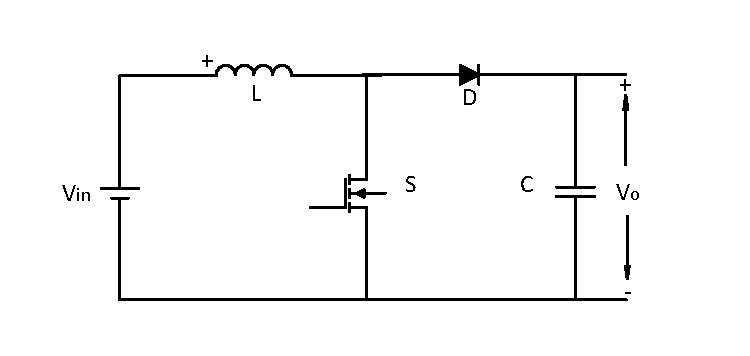
\includegraphics[width=\textwidth]{figures/aConventionalBoost/ConventionalBoostConverter.pdf}
    \caption{Conventional Boost Converter}
	\label{fig:ConventionalBoost}
\end{figure}

\section{Operation Modes}\label{sec:SON}

Switch ON:

When the switch is ON,
the inductor is being charged and the capacitor discharges over the load resistor.

\begin{figure}[H]
   \centering
   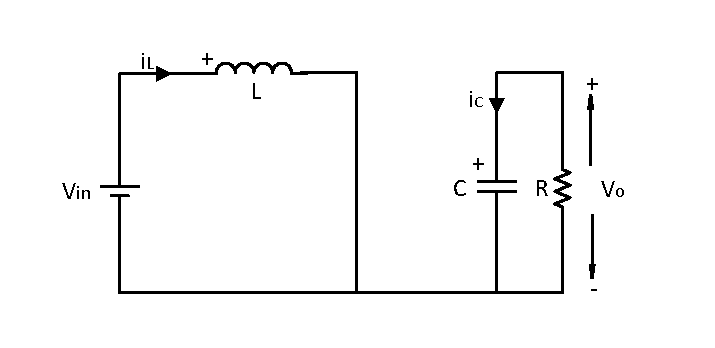
\includegraphics[width=\textwidth]{figures/aConventionalBoost/ConventionalBoostConverterON.pdf}
    \caption{Conventional Boost Converter Switch ON}
	\label{fig:ConventionalBoostONN}
\end{figure}

In this case we have:
\begin{equation}
	V_L = V_{in}
	\label{eq:pumpHeadModel}
\end{equation}
and
\begin{equation}
	V_C = V_R
	\label{eq:pumpHeadMode2}
\end{equation}
The capacitor current discharges over the resistor:
\begin{equation}
	i_C = -\frac{V_o}{R}
	\label{eq:pumpHeadMode3}
\end{equation}


Switch OFF:

\begin{figure}[H]
   \centering
   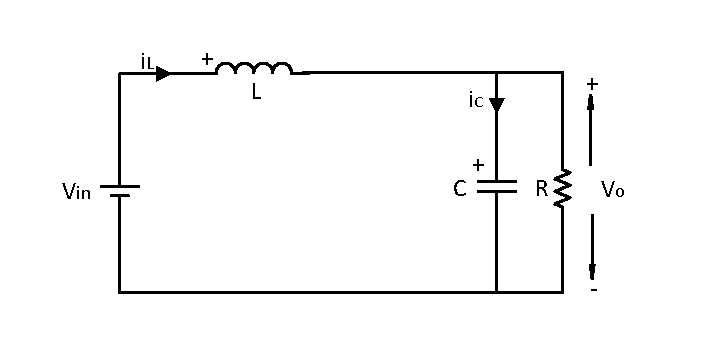
\includegraphics[width=\textwidth]{figures/aConventionalBoost/ConventionalBoostConverterOFF.pdf}
    \caption{Conventional Boost Converter Switch OFF}
	\label{fig:ConventionalBoostOFF}
\end{figure}

When the switch is OFF,
the capacitor is being charged and this is the mode when the boosting happens.

In this case we have:
\begin{equation}
	V_L = V_{in} - V_o
	\label{eq:pumpHeadModel}
\end{equation}

\begin{equation}
	i_C = i_L -\frac{V_o}{R}
	\label{eq:pumpHeadModel}
\end{equation}

\begin{figure}[H]
   \centering
   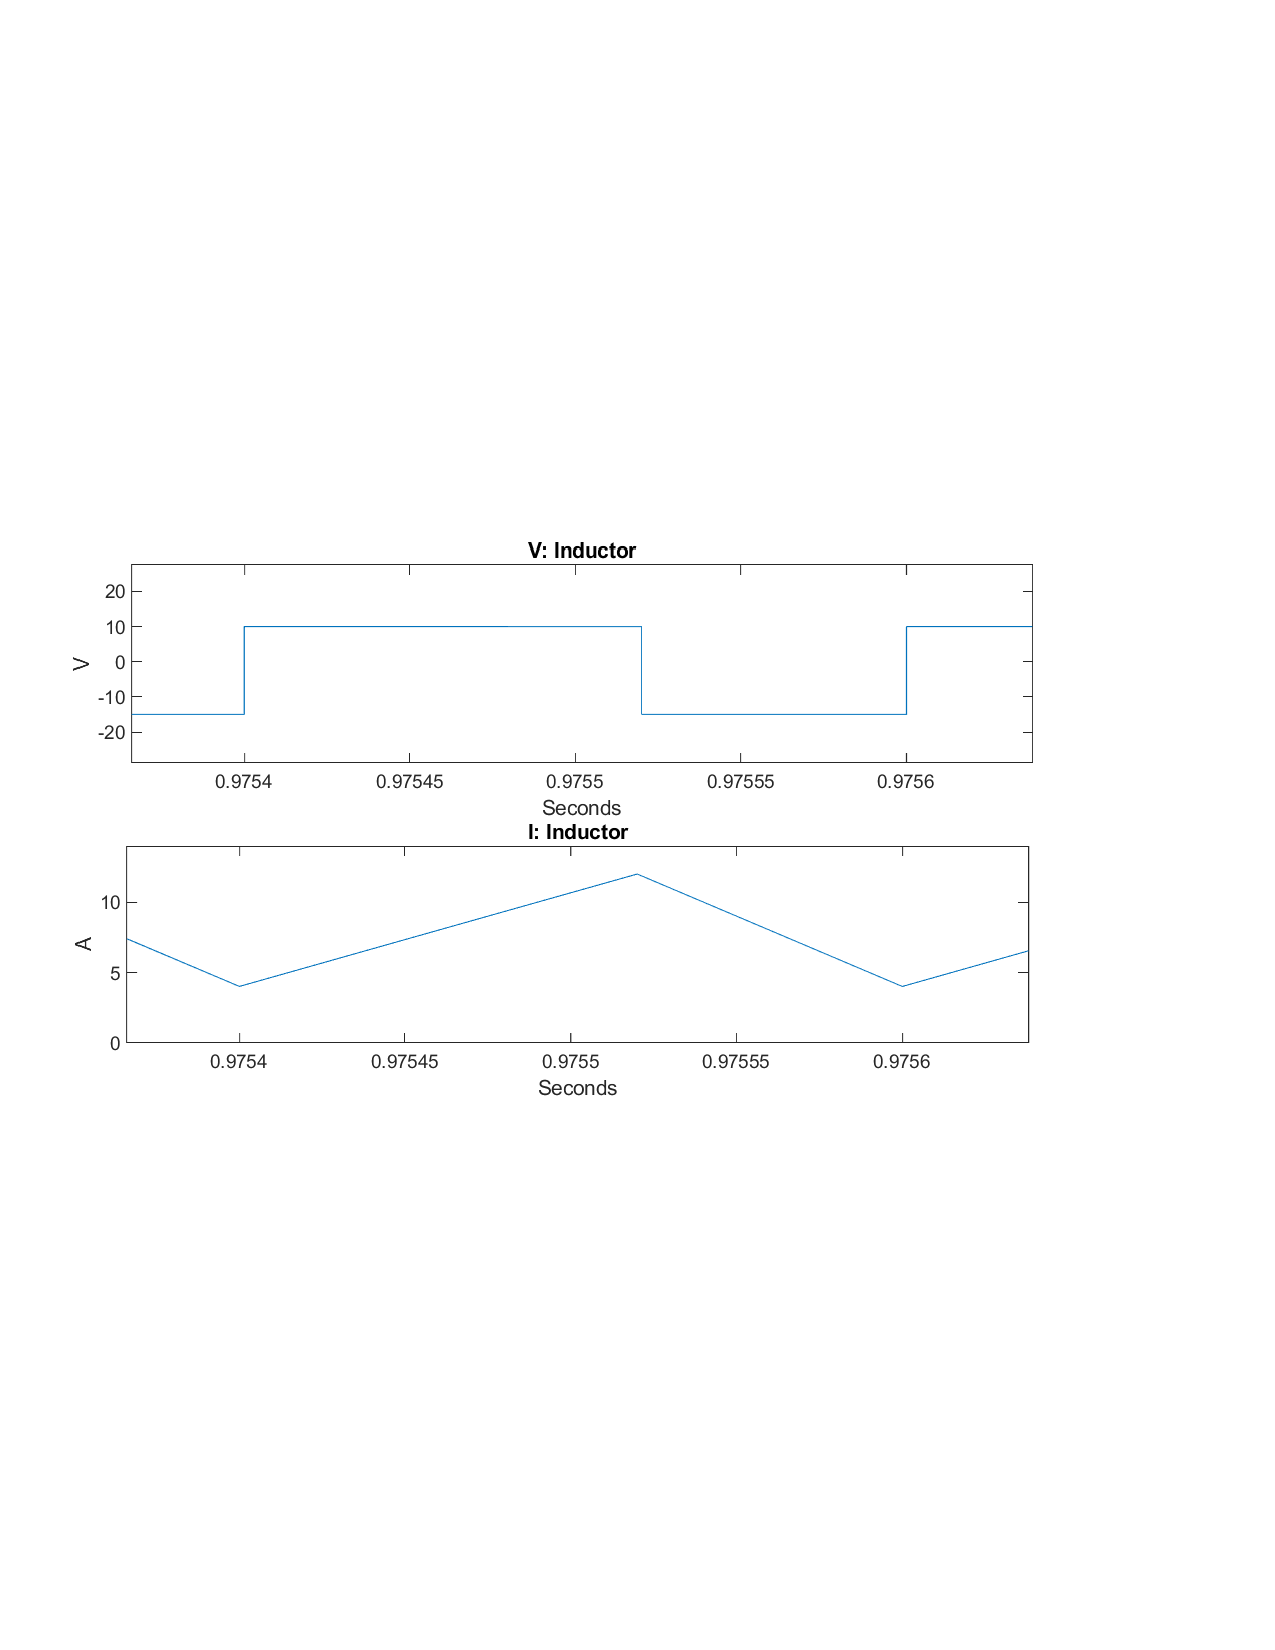
\includegraphics[width=\textwidth]{figures/aConventionalBoost/LvAndLi.pdf}
    \caption{CBC Inductor Wave Forms}
	\label{fig:ConventionalBoostOFF}
\end{figure}

Based on inductor volt-second balance, the convertion ratio can be calculated:

\begin{equation}
	V_{in}D + (V_{in}-V{out})(1-D) = 0
	\label{eq:pumpHeadModel}
\end{equation}

\begin{equation}
	\frac{V_o}{V_{in}} = \frac{1}{1-D}
	\label{eq:pumpHeadMode5}
\end{equation}